%------------------------------------------------------------
% DEFINITIONS AND HEADERS -- IGNORE THIS
%------------------------------------------------------------
\documentclass{article}
\usepackage[top=2.2cm, bottom=2.1cm, left=2.2cm, right=2.2cm]{geometry}
\usepackage[utf8]{inputenc}
\usepackage{algpseudocode}
\usepackage{csvsimple}
\usepackage{booktabs}
\usepackage{graphicx}
\usepackage{float}
\usepackage{listings}
\usepackage{xcolor}
% Get better typography
\usepackage[protrusion=true,expansion=true]{microtype}  
% For algorithms
\usepackage[boxruled,linesnumbered,vlined,inoutnumbered]{algorithm2e}
\SetKwInOut{Parameter}{Parameters}
% For basic math, align, fonts, etc.
\usepackage{amsmath}
\usepackage{amsthm}
\usepackage{amssymb}
\usepackage{mathtools}
\usepackage{mathrsfs}
\usepackage{rotating}
\usepackage{tabularx}
\usepackage{booktabs}
\usepackage{soul}
\usepackage{changepage}
\usepackage{gensymb} % For \degree
\usepackage{lscape}
% For \thead to make line breaks in tables
\usepackage{array}
\usepackage{makecell}
\renewcommand\theadalign{bc}
\renewcommand\theadfont{\bfseries}
\renewcommand\theadgape{\Gape[4pt]}
\renewcommand\cellgape{\Gape[4pt]}
\usepackage{courier} % For \texttt{foo} to put foo in Courier (for code / variables)
\usepackage{lipsum} % For dummy text
% For images
\usepackage{graphicx}
\usepackage{subcaption}
\usepackage[space]{grffile} % For spaces in image names
% For bibliography
\usepackage[round]{natbib}
% For color
\usepackage{xcolor}
\definecolor{light-grey}{rgb}{0.9,0.9,0.9}
\definecolor{dark-red}{rgb}{0.4,0.15,0.15}
\definecolor{dark-blue}{rgb}{0,0,0.7}
\definecolor{darkblue}{rgb}{0,0,.6}
\definecolor{darkred}{rgb}{.58,0,0}
\definecolor{brighterred}{rgb}{.745,0,0}
\definecolor{darkgreen}{rgb}{0,.6,0}
\definecolor{red}{rgb}{.98,0,0}
\usepackage{environ}
% Only show sections in table of contents and rename
\setcounter{tocdepth}{2}
\renewcommand{\contentsname}{Table of Contents}
% For links (e.g., clicking a reference takes you to the phy)
\usepackage{hyperref}
\hypersetup{
    colorlinks, linkcolor={dark-blue},
    citecolor={dark-blue}, urlcolor={dark-blue}
}
\newcommand{\HIGHLIGHT}[1]{\textcolor{blue}{\textbf{#1}}}
% \newcommand{\Solution}[1]{{\color{blue} \paragraph{\bf $\bigstar $ SOLUTION:} { \sf
%     #1} \bigskip}}
\newcommand{\TODO}[1]{\textcolor{blue}{\textbf{{#1}}}}
\newcommand{\POINTS}[1]{\textcolor{purple}{\textbf{{#1}}}}
\providecommand{\mathcolor}[2]{\textcolor{#1}{#2}}
% My definition of "summary boxes" (see below)
\usepackage[most]{tcolorbox}
\definecolor{boxgray}{rgb}{0.95, 0.95, 0.95}
\definecolor{boxblue}{rgb}{0.941, 0.941, 0.98}
\definecolor{boxpink}{rgb}{1.0, 0.93, 0.93}
\definecolor{boxwhite}{rgb}{1.0, 1.0, 1.0}
%\definecolor{boxgreen}{rgb}{0.91, 0.96, 0.9}
\definecolor{boxgreen}{rgb}{0.92, 0.96, 0.92}
\newtcolorbox{mybox}[1][boxwhite]{%
  enhanced,
  boxrule=0.5pt,
  colframe=black,
  colback=#1,
  sharp corners,
  width=\linewidth,
  left=1em,
  right=1em,
  top=0.5em,
  bottom=0.5em,
  boxsep=0pt,
  before skip=1em,
  after skip=0.85em,
}

\lstdefinestyle[style=filetree]{../../filetree.txt}{
  basicstyle=\ttfamily\small,
  breaklines=true,
  columns=fullflexible,
  frame=single,
  backgroundcolor=\color{gray!5},
  keepspaces=true
}
%------------------------------------------------------------





\begin{document}
%-----------------
%   Homework 4
%-----------------
\newpage
\vspace*{1cm}
\begin{center}
    \begin{Large}
    COMPSCI 589 Homework 4 - Spring 2026
    \end{Large}
    \\
    \vspace{0.15cm}
    Due \textcolor{darkred}{\textbf{April 30}}, 11:55 pm Eastern Time
\end{center}
\addcontentsline{toc}{subsection}{\textbf{Homework 4}}






%-------- Instructions --------------------------

\vspace{0.5cm}
\section*{Instructions}
\vspace{0.5cm}

\begin{itemize}
    \item This homework assignment consists of a programming part. 
    \item While you may discuss problems with your peers (e.g., to discuss high-level approaches), you must answer the questions on your own and implement all solutions independently. In your submission, do explicitly list all students with whom you discussed this assignment. 
    \item Submissions must be typed. You must use \LaTeX~to prepare your submission. Handwritten and scanned submissions will not be accepted. 
    \item The written report, including your answers, plots, and analysis, should be submitted on Gradescope as a PDF via the appropriate submission link. The source code should be submitted as a single .zip file through the separate programming assignment link on Gradescope.
    \item We strongly encourage using Python 3 for your homework code. You may use other languages. In either case, you \textit{must} provide clear instructions for running your code and reproducing your experiments. 
    \item You \textit{may not} use any machine learning-specific libraries in your code, e.g., TensorFlow, PyTorch, or machine learning algorithms implemented in scikit-learn (though you \textit{may} use other functions provided by this library, such as one that splits a dataset into training and testing sets). You may also use libraries such as numpy and matplotlib. If you are not certain whether a specific library is allowed, do ask us.
    \item All submissions will be checked for plagiarism using two independent plagiarism-detection tools. Renaming variable or function names, moving code within a file, etc., are all strategies that \textit{do not} fool the plagiarism-detection tools we use. Your code will also be compared with submissions from your classmates and with publicly available implementations online. 
    \item \textcolor{red}{If you get caught, all penalties mentioned in the syllabus \textit{will} be applied---which may include directly failing the course with a letter grade of ``F''}.
    
    \vspace{0.3cm}
    \noindent\rule{\linewidth}{0.5pt}
    \vspace{0.025cm}
    \item The automated system will not accept assignments after 11:55 pm on April 30.
    \item The TeX file for this homework (which you should use to write your solutions in \LaTeX), as well as the datasets you will investigate and two reference output files you can use to debug your implementation, are available on Canvas under ``\textit{Homework \#4 - Supporting Files}''. See below for more details.
\end{itemize}

% --------------------







%--------- High-Level Overview of the Homework --------------------------
\newpage
\noindent {\LARGE{\textbf{Programming Assignment}} \POINTS{[100 Points, total]}}
\vspace{0.75cm}

\noindent In this homework, you will be implementing the backpropagation algorithm to train a neural network. \textbf{Notice that you may \ul{not} use existing machine learning code for this problem: you must implement the learning algorithm entirely on your own and from scratch.} 

\vspace{0.75cm}

\noindent In this assignment, you will:

\begin{enumerate}
\item Implement the backpropagation algorithm to train a neural network. Your implementation should support networks with an \textit{adjustable} number of layers and neurons. For example, it should support training a neural network with two hidden layers, the first containing 5 neurons and the second containing 3 neurons, or a neural network with three hidden layers, each containing 4 neurons.
\item Implement the regularization mechanism discussed in class, which will be used here to help mitigate overfitting.
\item Evaluate your neural network using the \textit{stratified cross-validation} strategy that you implemented as part of a previous homework. We recommend using $k=5$ folds. Of these, $k-1$ folds will be used to train the neural network. The remaining fold (the one not used during training) will be used to evaluate the network's performance. You will then repeat this process, generating and evaluating $k$ neural networks. The final performance is the average of the performances computed across the $k$ folds.
\item Evaluate the performance of your neural network on two datasets as a function of three design decisions: the number of layers in the network, the number of neurons in each layer, and the regularization parameter.
\end{enumerate}

\vspace{0.75cm}

\noindent Each student is free to decide whether to implement the ``standard'' (non-vectorized) version of backpropagation or the vectorized version of backpropagation; that is, the version where all quantities relevant to training, such as predicted outputs, the value of the cost function $J$, and gradients, are computed using matrix multiplication operations. \textit{We strongly recommend that students complete this assignment using vectorization techniques.} This will significantly reduce the time required to train your neural network and will also lead to a more straightforward implementation of the backpropagation algorithm.

\vspace{0.75cm}

\noindent We are providing students with \textit{reference output files} that describe, for two simple neural networks, \textit{all} the relevant quantities computed by a correct implementation of the backpropagation algorithm, step by step. \textbf{These are intended to help you debug your implementation of the backpropagation algorithm.} These files describe, for example, the activation of each neuron when the network is presented with a particular training instance, the final output/prediction of the network for that instance, the $\delta$ value associated with each neuron, and the corresponding gradients of each weight in the network. Students \textit{should} use the information in these files to ensure that the quantities computed by their implementation of backpropagation match the expected values produced by a correct implementation of this learning algorithm. For example, if the gradients computed by a student's implementation do not match the expected values, the student should be able to quickly identify the first point during the execution of the algorithm where one of the quantities computed by their solution differs from the correct/expected one. This should facilitate debugging. More information about the \textit{reference output files} can be found in Section~\ref{correctness_verif}.





%--------- Description of Deliverables and Datasets/Experiments --------------------------
\newpage

\noindent {\LARGE{\textbf{Deliverables and Experiments}}}
\vspace{0.75cm}

\noindent The main objective of this homework is to study how the performance of a trained neural network is affected by \textit{\textbf{(i)}} the neural network architecture (i.e., the number of layers and neurons) and \textit{\textbf{(ii)}} the regularization parameter.
\vspace{0.1cm}

\noindent You should \ul{first} verify the correctness of your implementation by comparing the outputs it produces with the step-by-step examples we provide (see Section~\ref{correctness_verif}). After that, you will analyze two datasets. \textbf{Both datasets are included in the homework’s ``Supporting Files'' zip file on Canvas.}

\vspace{0.4cm}


\noindent The two datasets you will investigate are the following:
\vspace{0.4cm}

\noindent \textbf{(1) \textcolor{darkblue}{\ul{The Wisconsin Breast Cancer Diagnostic (WDBC) Dataset}}.}
\noindent The goal here is to train a classifier capable of predicting whether a breast mass is malignant or benign, based on features computed from a digitized image of a breast mass. The dataset is composed of 569 instances. Each instance is described by 30 \textit{numerical} attributes, and there are two classes.
\vspace{0.5cm}

\noindent \textbf{(2) \textcolor{darkblue}{\ul{The Loan Eligibility Prediction Dataset}}.}
\noindent Here, the goal is to automatically (and accurately) predict whether a given person should qualify for a loan. Each instance is described by 11 attributes, including the gender of the applicant, whether the applicant is married, their income, information about their credit history, etc. The binary target class to be predicted is whether a given applicant's request for a loan was approved or not. Notice that this dataset contains 7 \textit{categorical} attributes and 4 \textit{numerical} attributes. There is a total of 480 instances in the dataset. 


\vspace{0.5cm}

\begin{mybox}[boxpink] 
    $\star$ Note that some of the datasets above include \ul{\textbf{both}} categorical and numerical attributes. Algorithms such as neural networks (and others) require numerical inputs. The standard way to convert categorical inputs into numerical form is to use \textit{one-hot encoding}. For a quick and high-level introduction to one-hot encoding, as well as examples on how to use Scikit's libraries to perform this type of conversion, please visit this \href{https://datagy.io/sklearn-one-hot-encode}{website}.
\end{mybox}

\vspace{2.25cm}

\begin{mybox}[boxblue] 
\textbf{Important}: When implementing your neural network, do not forget to add a \textit{bias} input to each neuron, and make sure that updates to bias weights are handled correctly if regularization is used. For more information, see the slides from the corresponding lecture. Also, make sure to properly normalize the attributes of the training and test instances whenever necessary.
\end{mybox}

%
%

\begin{mybox}[boxblue] 
\textbf{Important}: You are free to choose between two simple stopping criteria. You may, for instance, \textit{(1)} stop if, after presenting all training instances to the network and updating its weights, the cost function $J$ improves by less than some small user-adjusted constant $\varepsilon$; or \textit{(2)} stop after a constant, pre-defined number $m$ of iterations, where each iteration consists of presenting all instances in the training set to the network, computing gradients, and updating the network's weights. You are free to choose which criterion to use.

\vspace{0.3cm}

In all questions below, do not forget to explicitly state which criterion you used and the corresponding hyperparameter (i.e., $\varepsilon$ or $m$). We encourage you to try different settings to identify the one that produces the best possible performance for your algorithm.
\end{mybox}

\vspace{1.25cm}





%----------- Steps for Verifying the Correctness of your Backprop Implementation ----------------------
\newpage
\section{Correctness Verification}
\label{correctness_verif}

\vspace{0.3cm}

\begin{enumerate}
\item You will first need to verify that your implementation of backpropagation is correct; i.e., that the gradients it computes are accurate. To do this, we are providing students with \textbf{two \ul{reference output files}}: \mbox{\emph{backprop\_example1.txt}} and \emph{backprop\_example2.txt}. Each file describes a specific neural network architecture and a minimal training set. It also shows, in detail, all intermediate quantities computed by the backpropagation algorithm, which you should compare with those produced by your implementation. These quantities include the activation of each neuron when the network is presented with a given input, the final predicted output (and the corresponding expected output), the network’s error/cost function $J$, the $\delta$ values for each neuron, and the gradients of all weights.

\looseness-1
\item You \textit{must} ensure that your implementation of backpropagation is correct. To do so, you should write a function capable of reproducing the quantities described in each of the two reference output files. This function should produce textual output (e.g., using simple \texttt{print} statements) indicating all relevant quantities computed by your implementation, similar to how they are presented in the provided reference output files.

\item As part of your solution to this assignment, you \textit{must} allow us to call this function; that is, the function that demonstrates that your code can reproduce the outputs presented in \emph{backprop\_example1.txt} and \emph{backprop\_example2.txt}, so that we can verify the correctness of your implementation. The output you generate does not need to be identical to that shown in the reference output files, but it should include at least, for each training instance and for both datasets, the activation of each neuron; the final predicted output of the network; the expected output; the cost $J$ associated with that instance; the $\delta$ values of each neuron and the gradients of all weights after the network is presented with that training instance; and the final regularized gradients after the backpropagation algorithm has processed all instances in the training set.

\end{enumerate}

\vspace{0.5cm}

\noindent \textcolor{darkblue}{\textbf{You should then:}} 

\begin{enumerate}
    \renewcommand{\labelenumi}{(\roman{enumi})}
    \item Include in your report clear instructions describing how we (the instructor, staff, and TAs) can run the function you implemented to demonstrate the correctness of your backpropagation algorithm; that is, the function that produces all the results and quantities described above.
    \item \ul{Present in your report the textual output produced by this function} for both provided reference output files. This part of the assignment is extremely important, and a non-trivial portion of your final grade will depend on whether we can verify that you implemented the backpropagation training algorithm correctly.
\end{enumerate}

\noindent We strongly recommend that you only start working on the next part of this assignment \textit{after} you have verified that your implementation of backpropagation is correct. Otherwise, it may be hard, or even impossible, for your neural network to properly learn solutions to the proposed problems.
\vspace{0.5cm}

\noindent The two reference output files we provide (\emph{backprop\_example1.txt} and \emph{backprop\_example2.txt}) are structured as follows: 

\begin{itemize}
\item The first line of each file specifies the regularization parameter, $\lambda$, that should be used. The next line describes the network structure, that is, the number of neurons in each layer. Recall that the first layer corresponds to the network's input layer and the last layer corresponds to the output layer. In the notation adopted here, the bias neuron is \textit{not} included in the neuron counts shown in this line.

\item Consider, for example, a neural network with two inputs, one hidden layer with 3 neurons, and one output. In this case, the second line of the provided files would define the network's structure as [2 3 1]. Notice, however, that your implementation \textit{should} include bias neurons and bias weights. We do not typically count them when specifying the architecture of a network because it is implicit that they are always used.

\item After this section of the file, you will encounter a description of the initial/current weights of the network. Each row represents the weights of a specific neuron in a particular layer; the weights of the $i$-th neuron are stored in the $i$-th row of the corresponding table/matrix. Recall that the first weight of each neuron corresponds to the bias weight connected to that neuron. 
\end{itemize}

\newpage

\noindent Consider the following simple neural network as an example:
\vspace{0.75cm}

\begin{figure}[!h]
    \centering
    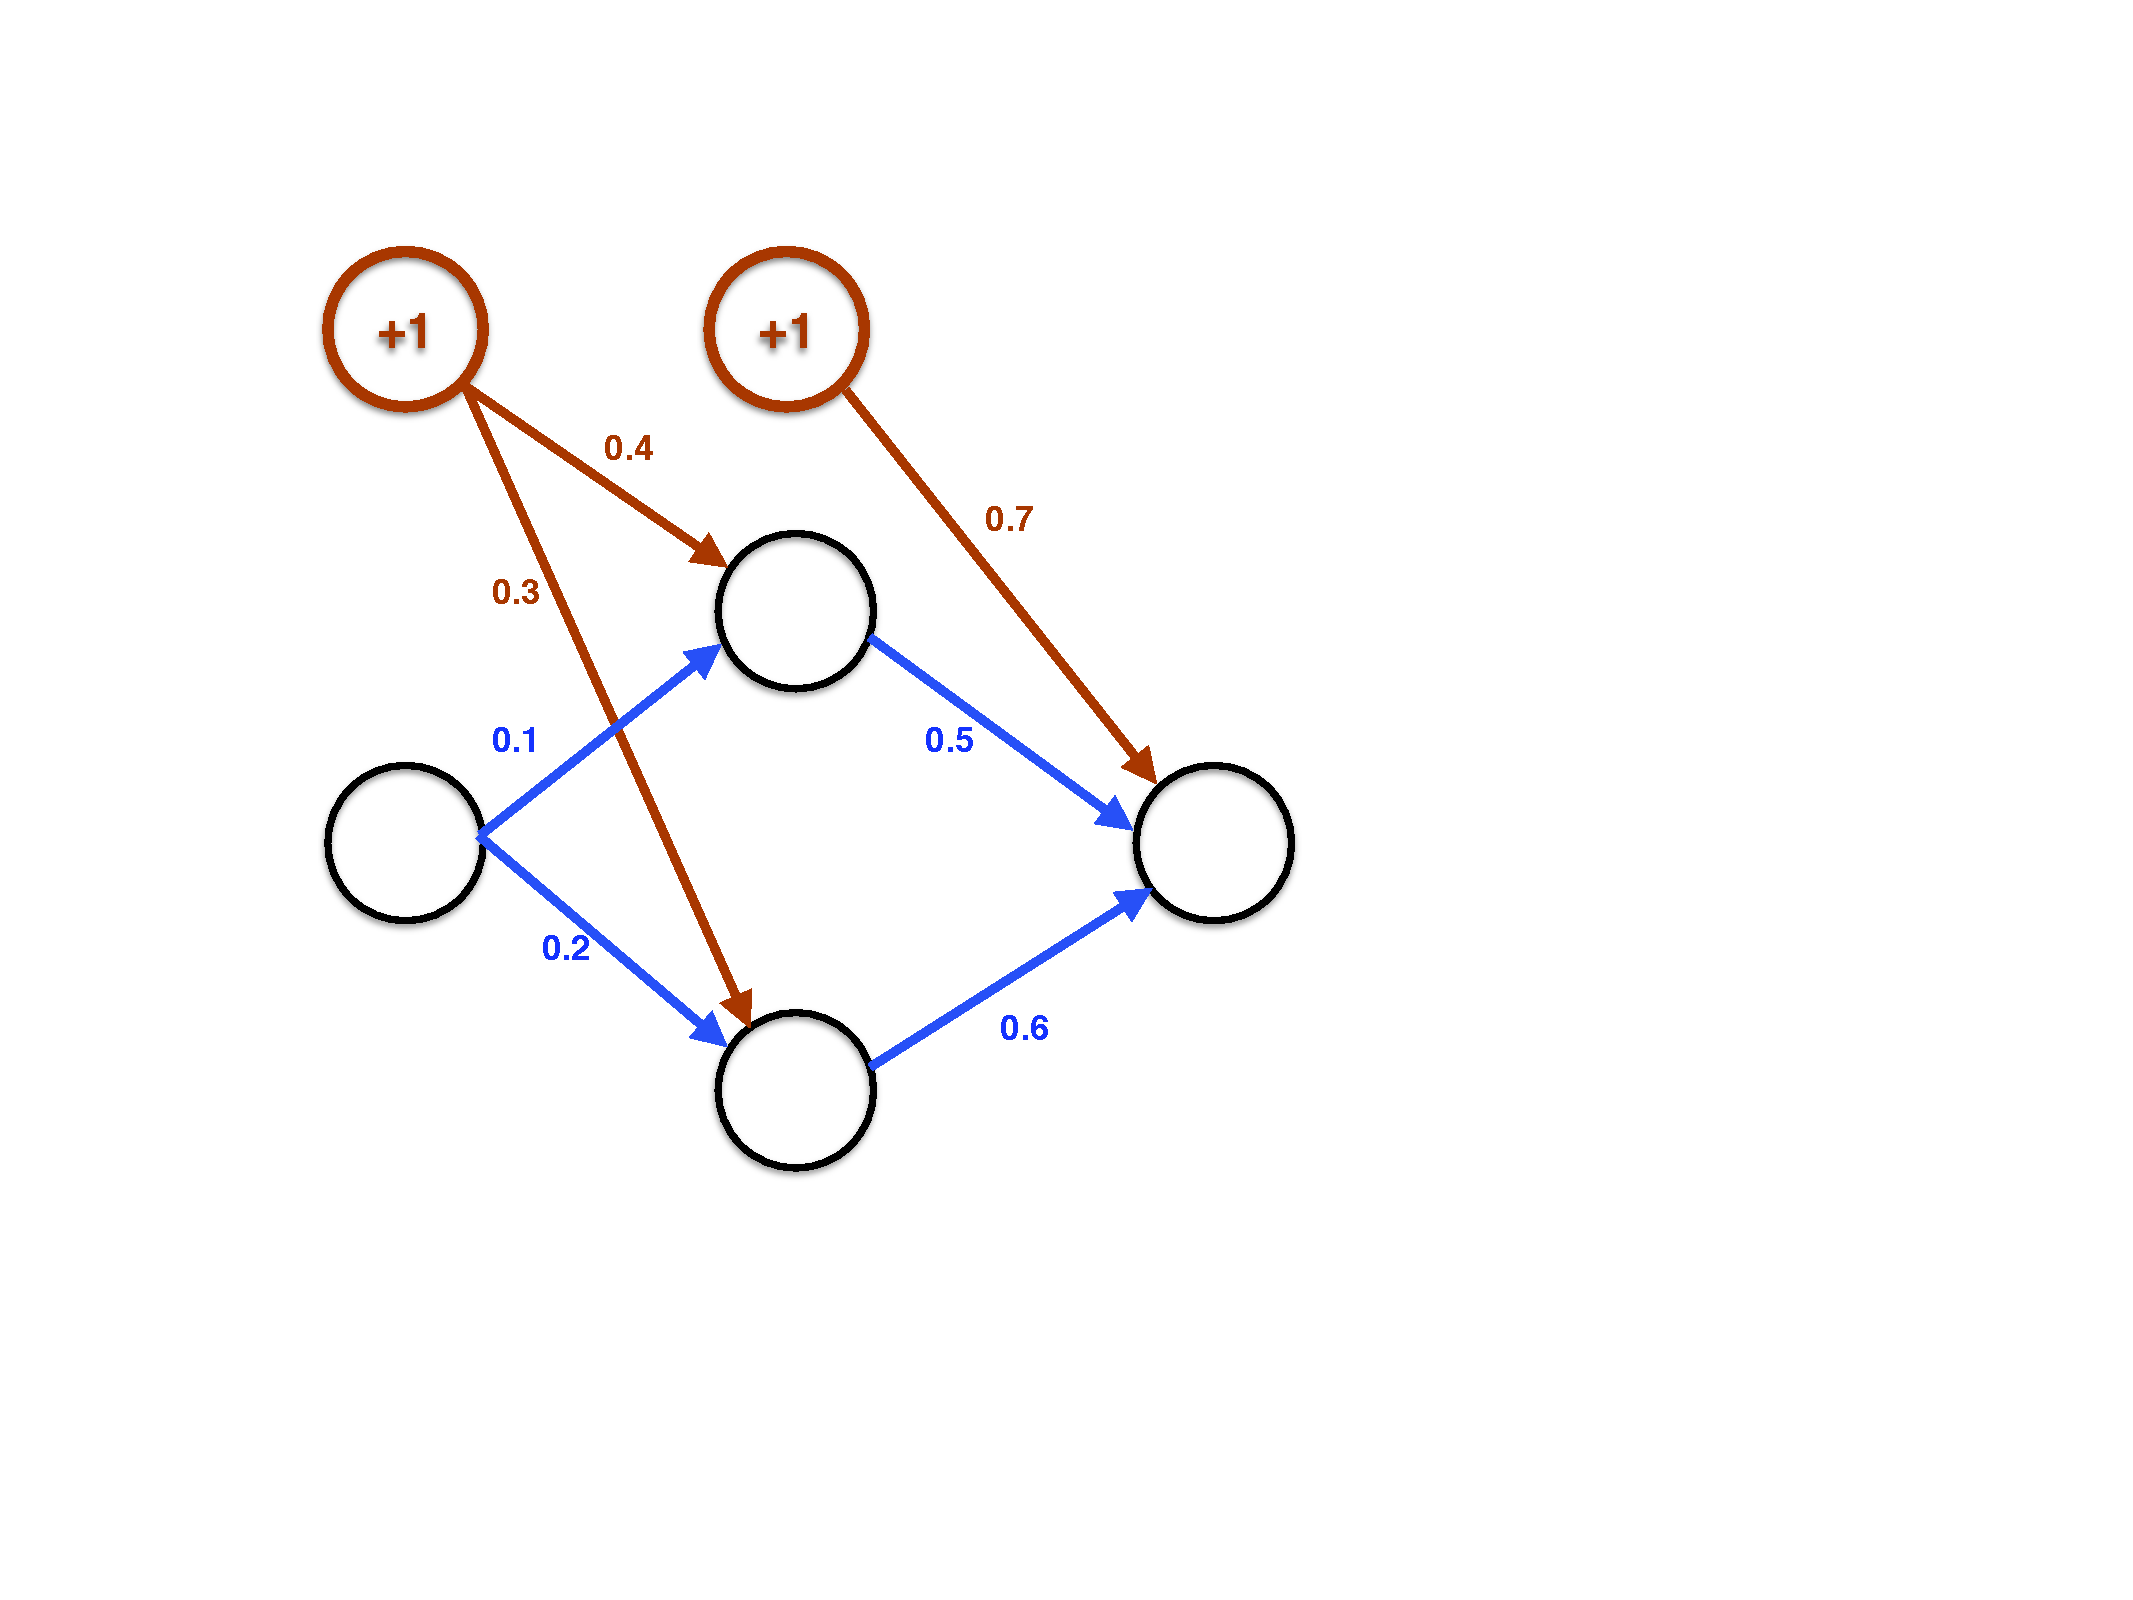
\includegraphics[width=0.4\columnwidth]{figures/HW4_network_example.pdf}
\end{figure}

\vspace{0.7cm}

\noindent The weights $\theta^{l=1}$ (Theta1) would be shown as follows:
%
\begin{verbatim}
 0.4 0.1
 0.3 0.2
\end{verbatim}

\vspace{0.4cm}

\noindent The weights $\theta^{l=2}$ (Theta2) would be shown as follows:    
%
\begin{verbatim}
 0.7 0.5 0.6
\end{verbatim}

\vspace{0.75cm}

\noindent After this section of the file, you will find a description of the inputs ($x$) and expected outputs ($y$) for each instance in the training set. The subsequent parts of the file show the intermediate quantities computed during forward propagation for each training instance. In particular, it reports the $z$ and $a$ values of each neuron (i.e., their activations), as well as the network's final prediction, $f(x)$, and the cost function $J$ associated with that instance.

\vspace{0.55cm}

\noindent The final section of each file presents all intermediate quantities computed during the backpropagation phase: the $\delta$ values of each neuron after processing a given training instance, and the gradients of all weights after that instance is processed. It then reports the final regularized gradients of all weights, computed using all training instances. As discussed in class, these gradients are used to update the network's weights so that it, on average, makes better predictions across all training examples in the dataset.








%------ Experiments and Analyses (i.e., Questions that should be answered) --------------------------
\newpage
\section{Experiments and Analyses}
\vspace{0.3cm}
\textcolor{darkblue}{\large \textbf{For each dataset, you should}}:
\vspace{0.25cm}


\begin{enumerate}
    \item Train a neural network and evaluate it using the stratified cross-validation technique discussed in class. You should train neural networks using different values of the regularization parameter, $\lambda$, and different network architectures. You may decide which architectures to evaluate. For example, you might test networks with 1, 2, 3, and 4 hidden layers, and vary the number of neurons per layer, such as 2, 4, 8, and 16.
    \item For each trained neural network, that is, for each combination of architecture and regularization that you tested, you should measure the resulting model's accuracy and F1-score.
    \item Based on these experiments, you should create, for each dataset and for each of the metrics described above, a table summarizing the results. In particular, report the value of each performance metric for every neural network configuration you tested, on both datasets. \textbf{You should test \textit{at least} 6 neural network architectures on each dataset.}
    \item Discuss (at a high level) what contributed most to improving performance: changing the regularization parameter; adding more layers; using deeper networks with many layers but few neurons per layer; or designing networks with few layers but many neurons per layer. Describe any patterns you may have observed. Also discuss whether there is a point at which constructing and training more ``sophisticated''/complex networks, that is, larger networks, no longer improves performance (or even worsens it).
    \item Based on the analyses above, discuss which neural network architecture you would select if you had to deploy such a classifier in practice. Explain your reasoning.
    \looseness-1
    \item After identifying the best neural network architecture for each dataset, train it again on the corresponding dataset and create a learning curve in which the $y$-axis shows the network's performance ($J$) on a test set and the $x$-axis shows the number of training samples provided to the network. This graph should illustrate the following idea: after showing 5 training examples to the network, what is its performance $J$ on the test set? After showing 10 training examples, what is its performance $J$ on the test set? If the network’s parameters and architecture are well adjusted, the graph should show that performance improves as the number of training examples increases; in particular, that $J$ \textit{decreases} as a function of the number of training instances presented to the network. Please also report the step size value, $\alpha$, that you used when training this network.

    \item We recommend, though this is \textit{not} required, that you train the network using the mini-batch gradient descent approach. You may manually select and adjust the mini-batch size you would like to use. Training a neural network in this way can significantly speed up the training process.
    
\end{enumerate}

\noindent\rule{\textwidth}{0.5pt}

\begin{mybox}[boxpink]
\begin{center}
\noindent \textbf{Some Hints (\underline{Important!})}
\end{center}

{\small
\begin{enumerate}
    \item Initialize the network's weights with small random numbers from -1 to +1, or with random numbers sampled from a Gaussian distribution with zero mean and variance equal to 1.
    \item When trying to identify effective network architectures, start by testing networks with few layers and few neurons. For example, you could begin with networks that have just one hidden layer. Increase the number of layers and/or the number of neurons per layer only when necessary.
    \item When training a given neural network architecture, try using larger step sizes, $\alpha$, at first. If you set $\alpha$ too small, the training process may become very slow or may prematurely converge to a bad local minimum, depending on the stopping criterion you use. By contrast, if the network's performance oscillates significantly during training when using large values of $\alpha$, you may be overshooting. In that case, decrease the value of $\alpha$. Repeat this process until you find the largest step size that can be used effectively; that is, the largest value that allows the weights to be updated fairly quickly but does not cause instability or divergence.
    \item After you identify a value of $\alpha$ that causes the network's performance to improve in a reasonably consistent way, check the performance (value of $J$) to which the network converges. If it is not satisfactory, your network architecture might be too simple, that is, the network may be underfitting. In that case, try increasing the number of layers and/or the number of neurons per layer. Then repeat the analysis above to evaluate different step sizes, $\alpha$.

\end{enumerate}
}

\end{mybox}

\newpage
\section*{HW Delivery}

\subsection*{HW Delivery 1: Correctness Verification}

\begin{figure}[htbp]
\centering
\begin{minipage}{0.95\linewidth}
\lstinputlisting[style=filetree]{../../filetree.txt}
\end{minipage}
\caption{Code directory}
\label{fig:filetree}
\end{figure}


\noindent \textbf{Run command:}
\begin{itemize}
    \item Example 1: python exmaple\_1.py
    \item Example 2: python exmaple\_2.py
\end{itemize}

\noindent \textbf{Result:}

\noindent \text{Example 1 Result:}

Regularization parameter lambda=0.000

Initializing the network with the following structure (number of neurons per layer): [1 2 1]

Initial Theta1 (the weights of each neuron, including the bias weight, are stored in the rows):
0.40000  0.10000
0.30000  0.20000

Initial Theta2 (the weights of each neuron, including the bias weight, are stored in the rows):
0.70000  0.50000  0.60000

Training set
Training instance 1
x: [0.13000]
y: [0.90000]
Training instance 2
x: [0.42000]
y: [0.23000]

--------------------------------------------
Computing the error/cost, J, of the network
Processing training instance 1
Forward propagating the input [0.13000]
a1: [1.00000   0.13000]

z2: [0.41300   0.32600]
a2: [1.00000   0.60181   0.58079]

z3: [1.34937]
a3: [0.79403]

Predicted output for instance 1: [0.79403]
Expected output for instance 1: [0.90000]
Cost, J, associated with instance 1: 0.366

Processing training instance 2
Forward propagating the input [0.42000]
a1: [1.00000   0.42000]

z2: [0.44200   0.38400]
a2: [1.00000   0.60874   0.59484]

z3: [1.36127]
a3: [0.79597]

Predicted output for instance 2: [0.79597]
Expected output for instance 2: [0.23000]
Cost, J, associated with instance 2: 1.276

Final (regularized) cost, J, based on the complete training set: 0.82098

--------------------------------------------
Running backpropagation
Computing gradients based on training instance 1
delta3: [-0.10597]
delta2: [-0.01270   -0.01548]

Gradients of Theta2 based on training instance 1:
-0.10597  -0.06378  -0.06155

Gradients of Theta1 based on training instance 1:
-0.01270  -0.00165
-0.01548  -0.00201

Computing gradients based on training instance 2
delta3: [0.56597]
delta2: [0.06740   0.08184]

Gradients of Theta2 based on training instance 2:
0.56597  0.34452  0.33666

Gradients of Theta1 based on training instance 2:
0.06740  0.02831
0.08184  0.03437

The entire training set has been processed. Computing the average (regularized) gradients:
Final regularized gradients of Theta1:
0.02735  0.01333
0.03318  0.01618

Final regularized gradients of Theta2:
0.23000  0.14037  0.13756

\\
\noindent \text{Example 2 Result:}

(1). lambda=0.250

(2). Initial Theta1
0.42000  0.15000  0.40000
0.72000  0.10000  0.54000
0.01000  0.19000  0.42000
0.30000  0.35000  0.68000

(3). Initial Theta2
0.21000  0.67000  0.14000  0.96000  0.87000
0.87000  0.42000  0.20000  0.32000  0.89000
0.03000  0.56000  0.80000  0.69000  0.09000

(4). Initial Theta3
0.04000  0.87000  0.42000  0.53000
0.17000  0.10000  0.95000  0.69000

(5). Training set
Training instance 1
x: [0.32000   0.68000]
y: [0.75000   0.98000]

Training instance 2
x: [0.83000   0.02000]
y: [0.75000   0.28000]

(6.1). Training instance 1
a1: [1.00000   0.32000   0.68000]

z2: [0.74000   1.11920   0.35640   0.87440]
a2: [1.00000   0.67700   0.75384   0.58817   0.70566]

z3: [1.94769   2.12136   1.48154]
a3: [1.00000   0.87519   0.89296   0.81480]

z4: [1.60831   1.66805]
a4: [0.83318   0.84132]

Predicted f(x): [0.83318   0.84132]
Real value 1: [0.75000   0.98000]
* Cross-entropy J(1): 0.791

(6.2). Training instance 2
a1: [1.00000   0.83000   0.02000]

z2: [0.55250   0.81380   0.17610   0.60410]
a2: [1.00000   0.63472   0.69292   0.54391   0.64659]

z3: [1.81696   2.02468   1.37327]
a3: [1.00000   0.86020   0.88336   0.79791]

z4: [1.58228   1.64577]
a4: [0.82953   0.83832]

Predicted f(x): [0.82953   0.83832]
Real value 2: [0.75000   0.28000]
* Cross-entropy J(2): 1.944

* Final (regularized) cost, J: 1.90351

(7) Backpropagation
Gradients on instance 1
delta4: [0.08318   -0.13868]
delta3: [0.00639   -0.00925   -0.00779]
delta2: [-0.00087   -0.00133   -0.00053   -0.00070]

Gradients of Theta3 based on training instance 1:
0.08318  0.07280  0.07427  0.06777
-0.13868  -0.12138  -0.12384  -0.11300

Gradients of Theta2 based on training instance 1:
0.00639  0.00433  0.00482  0.00376  0.00451
-0.00925  -0.00626  -0.00698  -0.00544  -0.00653
-0.00779  -0.00527  -0.00587  -0.00458  -0.00550

Gradients of Theta1 based on training instance 1:
-0.00087  -0.00028  -0.00059
-0.00133  -0.00043  -0.00091
-0.00053  -0.00017  -0.00036
-0.00070  -0.00022  -0.00048

Gradients on instance 2
delta4: [0.07953   0.55832]
delta3: [0.01503   0.05809   0.06892]
delta2: [0.01694   0.01465   0.01999   0.01622]

Gradients of Theta3 based on training instance 2:
0.07953  0.06841  0.07025  0.06346
0.55832  0.48027  0.49320  0.44549

Gradients of Theta2 based on training instance 2:
0.01503  0.00954  0.01042  0.00818  0.00972
0.05809  0.03687  0.04025  0.03160  0.03756
0.06892  0.04374  0.04775  0.03748  0.04456

Gradients of Theta1 based on training instance 2:
0.01694  0.01406  0.00034
0.01465  0.01216  0.00029
0.01999  0.01659  0.00040
0.01622  0.01346  0.00032

Final regularized gradients of Theta1:
0.00804  0.02564  0.04987
0.00666  0.01837  0.06719
0.00973  0.03196  0.05252
0.00776  0.05037  0.08492

Final regularized gradients of Theta2:
0.01071  0.09068  0.02512  0.12597  0.11586
0.02442  0.06780  0.04164  0.05308  0.12677
0.03056  0.08924  0.12094  0.10270  0.03078

Final regularized gradients of Theta3:
0.08135  0.17935  0.12476  0.13186
0.20982  0.19195  0.30343  0.25249

\newpage
\subsection*{HW Delivery 2: WDBC Experiments and analysis}

\noindent \textbf{(1) \& (2) \& (3)}

\begin{table}[htbp]
\centering
\caption{WDBC Result}
\csvautobooktabular{../result/wdbc_result.csv}
\end{table}

\noindent \textbf{(4)}

\noindent For the WDBC dataset, increasing model complexity did not improve performance. The best results came from single-hidden-layer networks, such as 30-2-1 and 30-4-1, which achieved the highest accuracy of 0.979 and an F1 score of 0.983. Increasing the number of neurons or adding more layers yielded almost no improvement.\\

\noindent The impact of changing regularization parameters was also minimal. For simpler network architectures, results were very similar across most $\lambda$ values.\\

\noindent Deeper networks performed worse, such as 30-16-8-4-2-1, which saw a significant drop in both accuracy and F1-score. Beyond a certain point, increasing the complexity of the network drops performance.\\

\noindent \textbf{(5)}

\noindent \text{Choosen architecture: [30-2-1] with $\lambda$: 0.01}

\noindent \text{Reason:}
\begin{itemize}
    \item Highest accuracy: 0.979
    \item Highest F1-score: 0.983
    \item Simple model, fast to train
\end{itemize}

\noindent \textbf{(6)}

\begin{figure}[H]
\centering
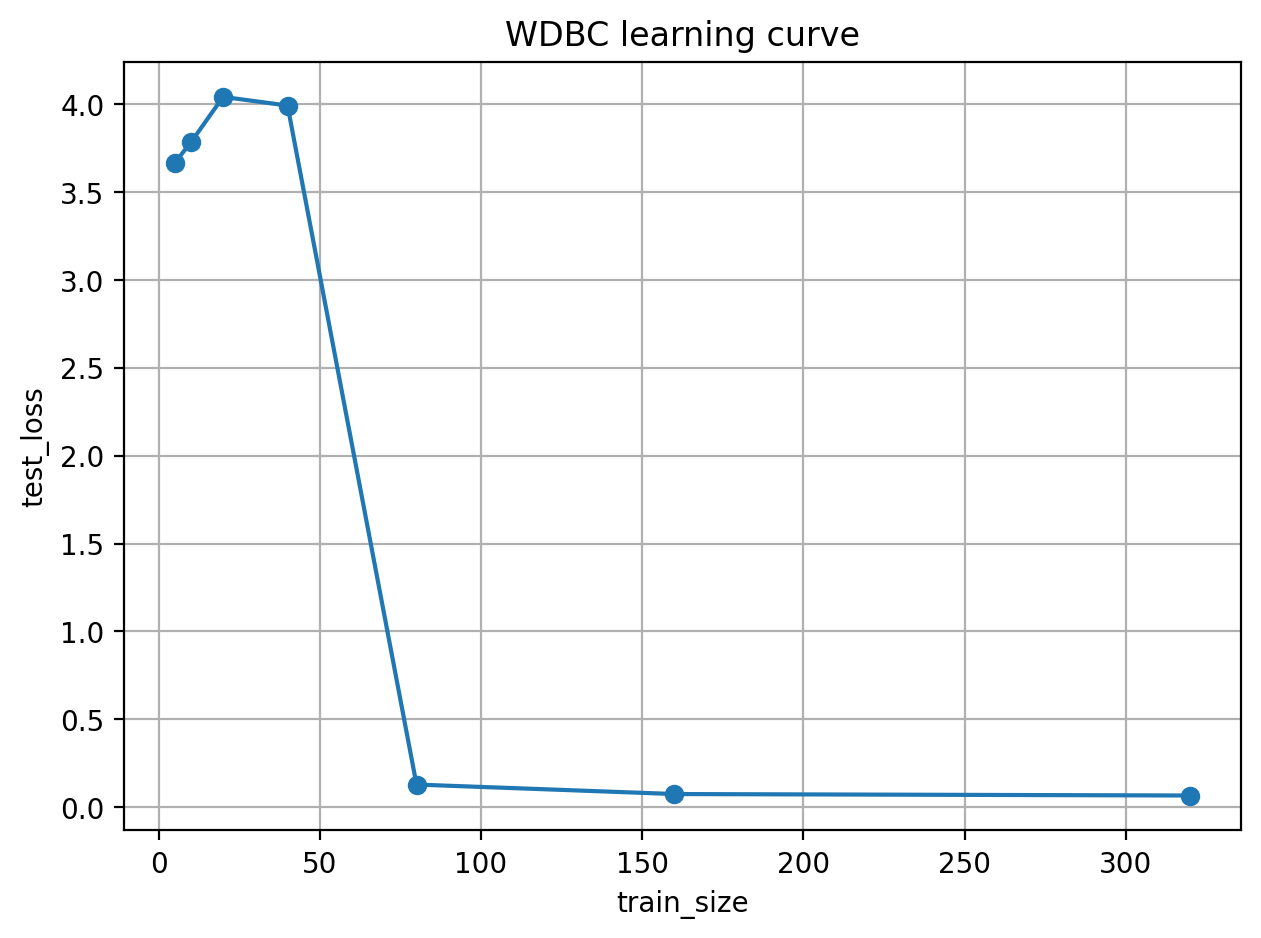
\includegraphics[width=0.8\textwidth]{../picture/wdbc_learning_curce.png}
\caption{Learning Curve for WDBC}
\label{fig:wdbc-learning-curve}
\end{figure}

\begin{itemize}
    \item Stopping criterion: epoch: 10000
    \item learning\_rate: 0.05
\end{itemize}

\newpage

\subsection*{HW Delivery 3: Loan Experiments and analysis}


\noindent \textbf{(1) \& (2) \& (3)}

\begin{table}[htbp]
\centering
\caption{Loan Result}
\csvautobooktabular{../result/loan_result.csv}
\end{table}

\noindent \textbf{(4)}

\noindent For the Loan dataset, regularization has a significant impact on performance. In many network architectures, increasing λ to 0.30 improves accuracy and F1-score.\\

\noindent Increasing the number of neurons or adding more layers did not improve performance. Simple networks, such as the 21-2-1 architecture, performed on par with many deeper models.\\

\noindent The most important factor is using an appropriate regularization value.\\

\noindent \textbf{(5)}

\noindent \text{Choosen architecture: [21-2-1] with $\lambda$: 0.3}

\noindent \text{Reason:}
\begin{itemize}
    \item Highest accuracy: 0.798
    \item Highest F1-score: 0.869
    \item Simple model, fast to train
\end{itemize}

\noindent \textbf{(6)}

\begin{figure}[H]
\centering
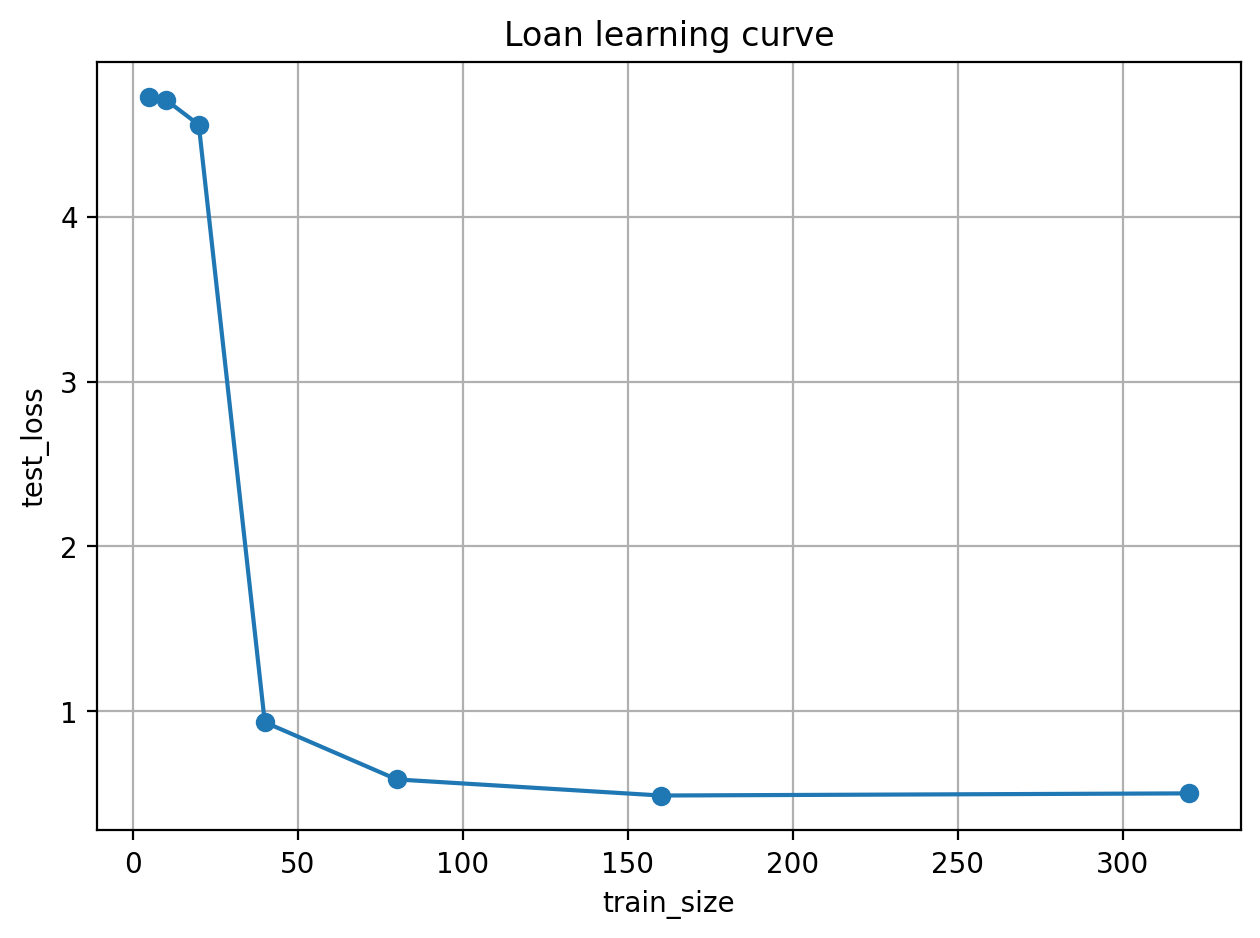
\includegraphics[width=0.8\textwidth]{../picture/loan_learning_curce.png}
\caption{Learning Curve for Loan}
\label{fig:loan-learning-curve}
\end{figure}

\begin{itemize}
    \item Stopping criterion: epoch: 20000
    \item learning\_rate: 0.05
\end{itemize}

\newpage

\subsection*{HW Delivery 4: Raisins Experiments and analysis}

\noindent \textbf{(1) \& (2) \& (3)}

\begin{table}[htbp]
\centering
\caption{Raisins Result}
\csvautobooktabular{../result/raisian_result.csv}
\end{table}


\noindent \textbf{(4)}

\noindent For the Raisin dataset, most network architectures performed similarly. The best results were achieved with a 7-16-8-4-1 architecture, $\lambda$ = 0.01, accuracy: 0.872, and F1-score: 0.867.\\

\noindent Changing the regularization parameters has some effect, but overall it is not significant.\\

\noindent Increasing the number of layers moderately is helpful, with the 7-16-8-4-1 architecture performing best. However, making the network deeper does not help. The most complex architecture, 7-16-8-4-2-1, performs poorly under certain regularization parameters.\\

\noindent \textbf{(5)}

\noindent \text{Choosen architecture: [7-16-8-4-1] with $\lambda$: 0.01}

\noindent \text{Reason:}
\begin{itemize}
    \item Highest accuracy: 0.872
    \item Highest F1-score: 0.867
\end{itemize}

\noindent \textbf{(6)}

\begin{figure}[H]
\centering
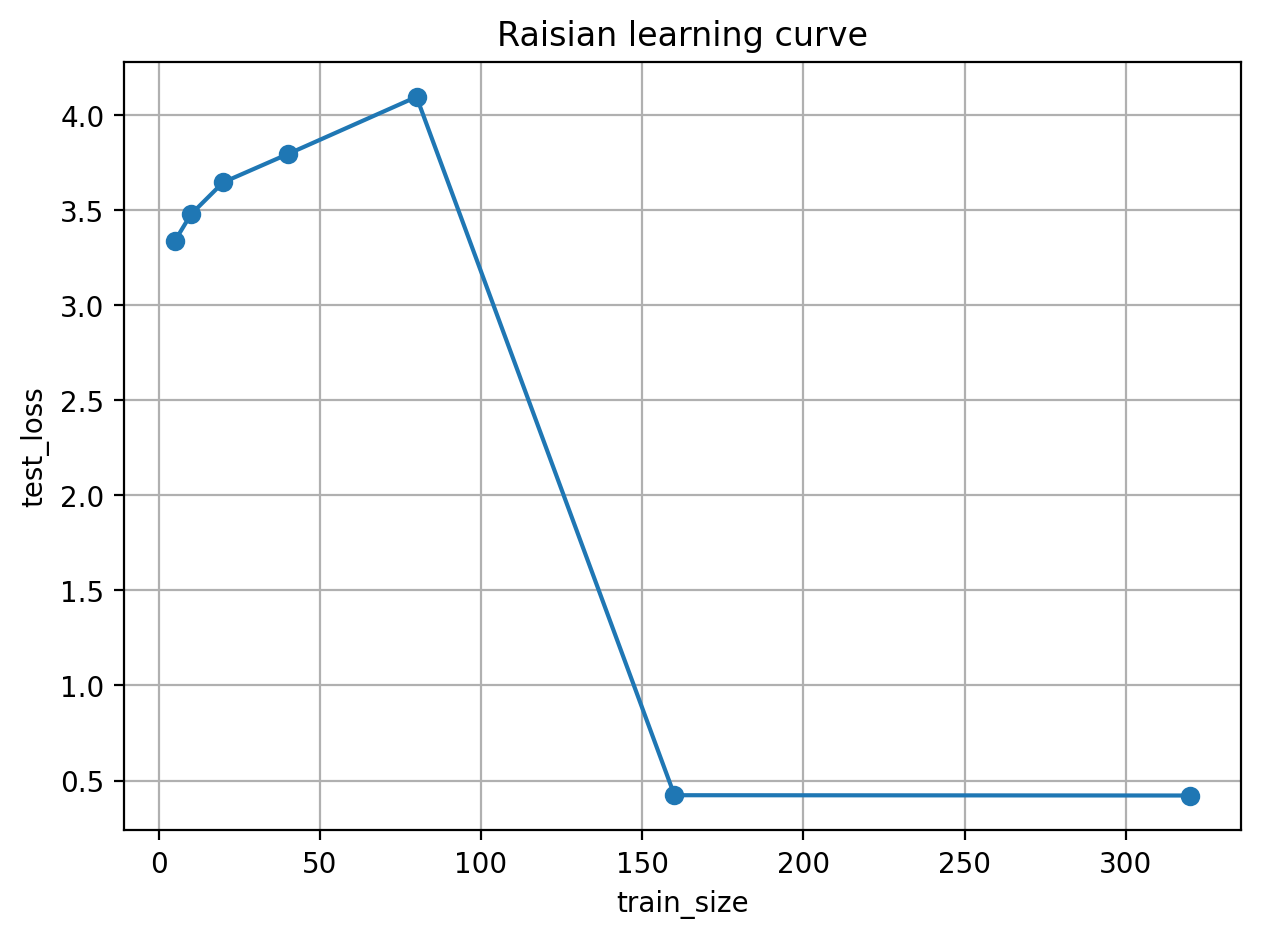
\includegraphics[width=0.8\textwidth]{../picture/Raisian_learning_curce.png}
\caption{Learning Curve for Raisins}
\label{fig:Raisians-learning-curve}
\end{figure}

\begin{itemize}
    \item Stopping criterion: epoch: 30000
    \item learning\_rate: 0.05
\end{itemize}

\newpage


\subsection*{HW Delivery 5: Titanic Experiments and analysis}

\noindent \textbf{(1) \& (2) \& (3)}

\begin{table}[htbp]
\centering
\caption{Titanic Result}
\csvautobooktabular{../result/titan_result.csv}
\end{table}

\noindent \textbf{(4)}

\noindent For the Titanic dataset, increasing the number of neurons is helpful, but adding too many layers can harm performance. The best results come from a single-hidden-layer network with a 9-16-1 architecture, lambda: 0.1, accuracy: 0.808, and F1-score: 0.726.\\

\noindent For most network architectures, changing the regularization parameter has little effect.\\

\noindent Deeper networks do not outperform simpler ones. The most complex architecture, 9-16-8-4-2-1, performs significantly worse, with lower accuracy and a much lower F1-score.\\

\noindent \textbf{(5)}

\noindent \text{Choosen architecture: [9-16-1] with $\lambda$: 0.1}

\noindent \text{Reason:}
\begin{itemize}
    \item Highest accuracy: 0.808
    \item Highest F1-score: 0.726
    \item SImple model, fast to train
\end{itemize}

\noindent \textbf{(6)}

\begin{figure}[H]
\centering
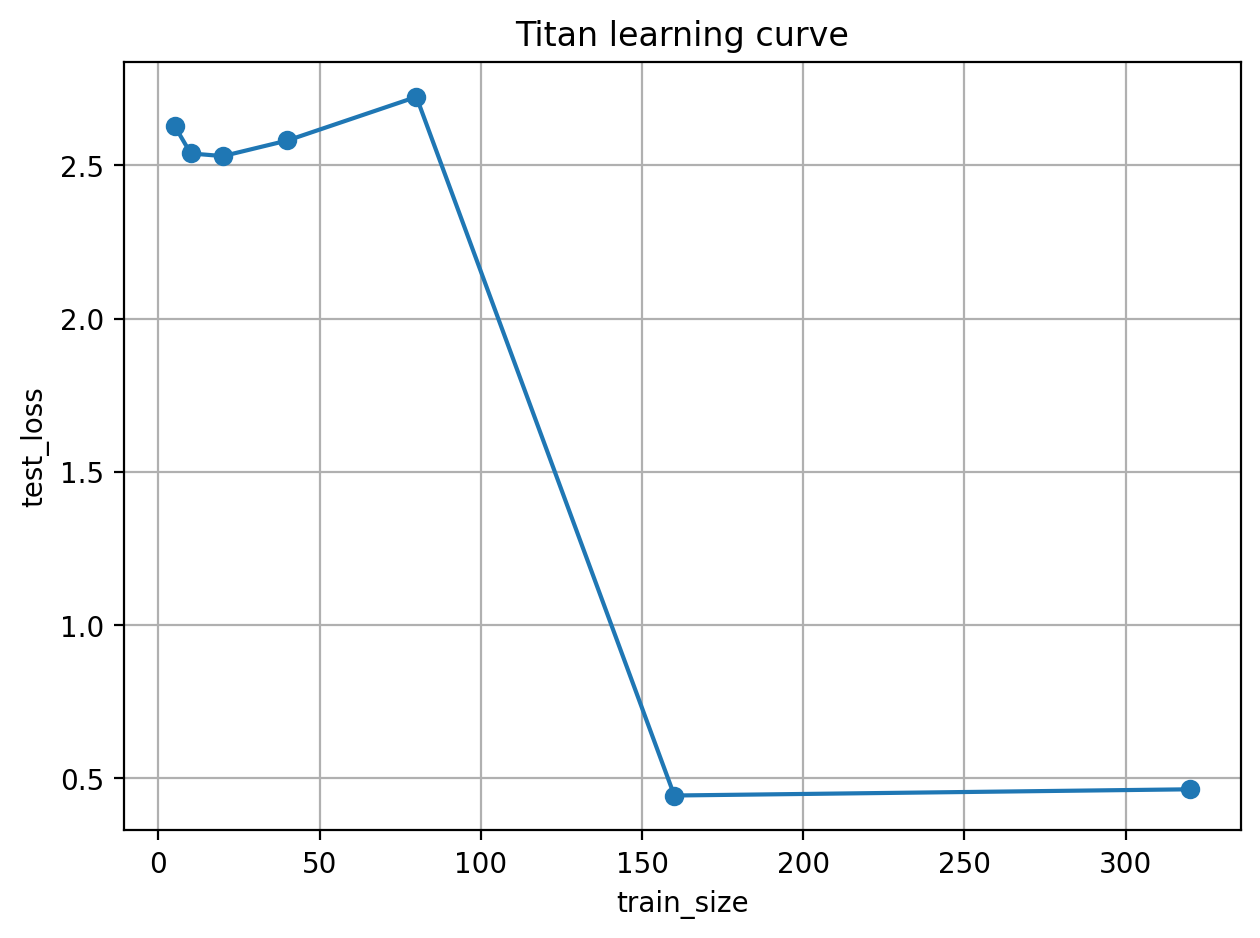
\includegraphics[width=0.8\textwidth]{../picture/Titan_learning_curce.png}
\caption{Learning Curve for Titanic}
\label{fig:Titanic-learning-curve}
\end{figure}

\\

\begin{itemize}
    \item Stopping criterion: epoch: 30000
    \item learning\_rate: 0.05
\end{itemize}

\newpage

\subsection*{HW Delivery 6: QE.3}







%-------- Extra Credit Questions --------------------------
\newpage
\noindent \textcolor{purple}{\textbf{\Large{Extra Credit Questions}}}
\vspace{0.6cm}

\noindent There are \ul{three} ways in which you may receive extra credit on this homework.




    %---- Extra Credit Question QE.1 ----------------------
    \vspace{1.25cm}
    \noindent \textbf{\HIGHLIGHT{[QE.1] [Extra Credit Question \raisebox{0.2ex}{\scalebox{0.8}{\textnormal{\#}}}1]~(\POINTS{13 Points})}} 
    \vspace{0.3cm}
    
    \noindent Analyze a third dataset: the \textcolor{darkred}{\textbf{\ul{Raisins Dataset}}}. The goal here is to use morphological features extracted from raisin images to classify each instance as either a Kecimen or a Besni raisin variety. The dataset contains 900 instances. Each instance is described by 7 \textit{numerical} features, and the dataset contains two classes. You should present the same analyses and graphs discussed above.
    %
    \begin{mybox}[boxgray] 
    This dataset can be found in the ``\textit{Supporting Files}'' zip file for this homework on Canvas.
    \end{mybox}

    


    %---- Extra Credit Question QE.2 ----------------------
    \vspace{1.25cm}
    \noindent \textbf{\HIGHLIGHT{[QE.2] [Extra Credit Question \raisebox{0.2ex}{\scalebox{0.8}{\textnormal{\#}}}2]~(\POINTS{13 Points})}} 
    \vspace{0.3cm}
    
    \noindent Analyze a fourth dataset: the \textcolor{darkred}{\textbf{\ul{Titanic Dataset}}}. On April 15, 1912, the largest passenger liner ever made collided with an iceberg during her maiden voyage. When the Titanic sank, it killed 1502 out of 2224 passengers and crew. One of the reasons the shipwreck resulted in such loss of life was that there were not enough lifeboats for the passengers and crew. Although luck was involved in surviving the sinking, some groups of people were more likely to survive than others. The goal here is to predict whether a given person was likely to survive this tragedy. The dataset contains data for 887 real passengers of the Titanic. Each row represents one person. The columns describe different attributes of the person, including whether they survived (the class/label), their age, their passenger class, sex, and the fare they paid. Notice that this dataset combines \textit{both numerical and categorical attributes}. You should present the same analyses and graphs discussed above.
    %
    \begin{mybox}[boxgray] 
    This dataset can be found in the ``\textit{Supporting Files}'' zip file for this homework on Canvas.
    \end{mybox}





    %---- Extra Credit Question QE.3 ----------------------
    \vspace{1.25cm}
    \noindent \textbf{\HIGHLIGHT{[QE.3] [Extra Credit Question \raisebox{0.2ex}{\scalebox{0.8}{\textnormal{\#}}}3]~(\POINTS{13 Points})}} 
    \vspace{0.3cm}
    
    \noindent Implement the method discussed in class that allows you to \textit{numerically} verify the gradients computed by your implementation of backpropagation. This will help you further ensure that all gradients computed by your implementation are correct, so that you can confidently trust your neural network training procedure. In your report, \ul{present} the estimated gradients for the two neural networks described in the provided reference output files. First, estimate and report the gradients using $\epsilon = 0.1$, and then using $\epsilon = 0.000001$. If you choose to complete this extra-credit task, please include the corresponding source code with your Gradescope submission.


\end{document}
